
\newcommand{\FIFODrawing}{
	\draw[draw=black,fill=white] (0.0,0) rectangle (1.5,0.75);
	\draw[draw=black] (0.75,0) -- (0.75,0.75);
	
	\node[mark size=1.4mm] at (0.38,0.35) {\pgfuseplotmark{*}};

	\fill [black!40,opacity=0.1] (0,0) -- (0,0.75) -- (-1.5,-0.25);
	\draw [black,densely dotted] (0,0) -- (0,0.75) -- (-1.5,-0.25) -- (0,0);
	
}

\newcommand{\FIFODrawingTwo}{
	\draw[draw=black,fill=white] (0,0) rectangle (1.5,0.75);
	\draw[draw=black] (0.75,0) -- (0.75,0.75);
	
	\node[mark size=1.4mm] at (0.38,0.35) {\pgfuseplotmark{*}};

	\fill [black!40,opacity=0.1] (0,0) -- (0,0.75) -- (-1.5,0.6);
	\draw [black,densely dotted] (0,0) -- (0,0.75) -- (-1.5,0.6) -- (0,0);
	
}

\newcommand{\FIFODrawingFour}{
	\draw[draw=black,fill=white] (1,0) rectangle (4,0.75);
        \draw[draw=black] (1.75,0)   -- (1.75,0.75);
        \draw[draw=black] (2.5,0) -- (2.5,0.75);
        \draw[draw=black] (3.25,0) -- (3.25,0.75);
	
	\node[mark size=1.4mm] at (1.38,0.35) {\pgfuseplotmark{*}};

        \fill [black!40,opacity=0.1] (-0.25,0.35) -- (1.0,0.75) -- (1.0,0.0);
        \draw [black,densely dotted] (-0.25,0.35) -- (1.0,0.75) -- (1.0,0.0) -- (-0.25,0.35);

}

\newcommand{\FIFODrawingThree}{
	\draw[draw=black,fill=white] (0,0) rectangle (1.5,0.75);
	\draw[draw=black] (0.75,0) -- (0.75,0.75);

	\fill [black!40,opacity=0.1] (0,0) -- (1.5,0) -- (1,-1.5);
	\draw [black,densely dotted] (0,0) -- (1.5,0) -- (1,-1.5) -- (0,0);
	
}

\newcommand{\memoryDDR}{
 \draw[fill=electricgreen!50] (0,0) rectangle (1,-7);
 \draw[line width=0.44mm] (0,-2) -- (1,-2);
 \draw[line width=0.15mm] (0,-1) -- (1,-1);
 \draw[line width=0.44mm] (0,-4) -- (1,-4);
 \draw[line width=0.15mm] (0,-3) -- (1,-3);
 \draw[line width=0.44mm] (0,-6) -- (1,-6);
 \draw[line width=0.15mm] (0,-5) -- (1,-5);

 \node[mark size=1.4mm] at (0.5,-2.5) {\pgfuseplotmark{*}};
 \node[mark size=1.4mm] at (0.5,-4.5) {\pgfuseplotmark{*}};

 \node at (0.5,-6.5) {\Huge \ldots};
}


\newcommand{\memoryDDRPointer}{
 \draw[fill=electricgreen!50] (0,0) rectangle (1,-7);
 \draw[line width=0.44mm] (0,-2) -- (1,-2);
 \draw[line width=0.15mm] (0,-1) -- (1,-1);
 \draw[line width=0.44mm] (0,-4) -- (1,-4);
 \draw[line width=0.15mm] (0,-3) -- (1,-3);

 \node[mark size=1.4mm] at (0.5,-0.5) {\pgfuseplotmark{*}};
 \node at (0.5,-6.5) {\Huge \ldots};
}

\newcommand{\FIFOMapping}{
\node  (fifoThree) at (1.5,0.9) {
		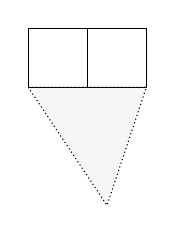
\begin{tikzpicture}
			\FIFODrawingThree
		\end{tikzpicture}
	};

\node (leg) at (1.5,-1.4) {\large \begin{tabular}{ll}$\Size(c)$&$=38$\,kB\\ $\Capacity(c)$&$=2$  \end{tabular}};
\node[ActorStyle] (convert) at (0,0) {\large $a_1$};
\node[ChannelStyle] (channelTwo) at (1.5,0) {\large $c_1$};
\node[ActorBroadcastStyle] (broadCastOne) at (3,0) {\large $a_2$};
\node[ChannelStyle] (channelThree) at (4.5,1.25) {\large $c_2$};
\node[ChannelStyle] (channelFour)  at (4.5,-1.25) {\large $c_3$};
\node[ActorStyle] (vertical) at (6,2) {\large $a_3$};
\node[ActorStyle] (horizontal) at (6,-2) {\large $a_4$ };

% now draw the arrows
\draw[ArrowStyle] (convert) -- (channelTwo);
\draw[ArrowStyle] (channelTwo) -- (broadCastOne);
\draw[ArrowStyle] (broadCastOne) -- (channelThree);
\draw[ArrowStyle] (broadCastOne) -- (channelFour);
\draw[ArrowStyle] (channelThree) -- (vertical);
\draw[ArrowStyle] (channelFour)  -- (horizontal);

%\draw [draw=black] (6,-3) rectangle (8,3);
\begin{scope}
\node[ChannelStyle] (channelFive) at (7.5,1.25) {\large $c_4$};
\node[ChannelStyle] (channelSix)  at (7.5,-1.25){\large $c_5$};

\draw[ArrowStyle] (vertical) -- (channelFive);
\draw[ArrowStyle] (horizontal) -- (channelSix);

\path [scope fading=west] (6.5,-3) rectangle (8,3);
\fill [fill=white] (6.5,-3) rectangle (8,3);

\end{scope}

\node  (fifoOne) at (6.0,-0.8) {
		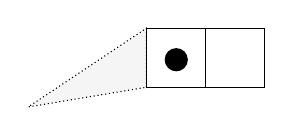
\begin{tikzpicture}
			\FIFODrawing
		\end{tikzpicture}
	};

\node  (fifoTwo) at (6.0,0.8) {
		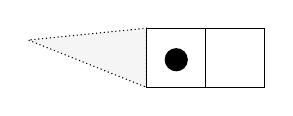
\begin{tikzpicture}
			\FIFODrawingTwo
		\end{tikzpicture}
	};


\node  (memDDR) at (10,0.5) {
		\begin{tikzpicture}
			\memoryDDR
		\end{tikzpicture}
	};

\node (legendStatic) at (4.5,-3.5){
                \resizebox{200pt}{!}{
                \begin{tikzpicture}
                        \legendApp
                \end{tikzpicture}}
        };

\node (legChannel1) at (8.75,3) {};
\node (legChannel2) at (8.75,1) {};
\node (legChannel3) at (8.75,-1){};

\draw [decorate,decoration={brace,amplitude=10pt,mirror,raise=4pt},yshift=0pt] (9.6,4) -- (9.6,2) node  [black,midway,xshift=0cm,yshift=-1cm] {};
\draw [decorate,decoration={brace,amplitude=10pt,mirror,raise=4pt},yshift=0pt] (9.6,2) -- (9.6,0) node  [black,midway,xshift=0cm,yshift=-1cm] {};
\draw [decorate,decoration={brace,amplitude=10pt,mirror,raise=4pt},yshift=0pt] (9.6,0) -- (9.6,-2) node [black,midway,xshift=0cm,yshift=-1cm] {};

\draw[->, >=triangle 60,dashed] (fifoOne.east) -- (legChannel3);
\draw[->, >=triangle 60,dashed] (fifoTwo.east) -- (legChannel2);
\draw (fifoThree.north) edge[bend  left=20,->,>= triangle 60,dashed] (legChannel1);
\node (leg) at (10,-3.5) {\Large \begin{tabular}{c}global memory \\ ($\GlobalMemory$) \end{tabular}};

\node[ChannelStyle]  at (4.5,1.25) {\large $c_2$};
\node[ChannelStyle]  at (4.5,-1.25) {\large $c_3$};
}


\newcommand{\FIFOPointerBasedMapping}{

%\draw[fill=green(munsell)!30,opacity=0.5,line width=0.25mm] (1.1,1.7) rectangle (4.9,-1.7);
%\draw[draw=black,line width=0.25mm] (1.1,1.7) rectangle (4.9,-1.7);
\draw[fill=green(munsell)!30,opacity=0.5,line width=0.25mm,radius=63pt] (3.3,0) circle;
\draw[draw=black,line width=0.25mm,radius=63pt] (3.3,0) circle;

\node (leg) at (0,-3) {\Large \begin{tabular}{ll} $\Size(c_{\{1,2,3\}})$ & $=38$\,kB\\ $\Capacity(c_{\{1,2,3\}})$ & $=4$ \end{tabular}};

%\node (leg) at (2.75,2.75) {\Large \color{black}{capacity($c_{\{1,2,3\}}$)$=8$}};
\node (leg) at (3.0,-1.5) {\huge \color{black}{$c_{\{1,2,3\}}$}};
%\begin{scope}[path fading]
\node[ActorStyle] (convert) at (0,0) {\Large $a_1$};
\node[ChannelStyle,opacity=0.3,text opacity=1] (channelTwo) at (1.5,0) {\large $c_1$};
\node[ActorBroadcastStyle,opacity=0.5,text opacity=1] (broadCastOne) at (3,0) {\large $a_2$};
\node[ChannelStyle,opacity=0.3,text opacity=1] (channelThree) at (4.5,1.25) {\Large $c_2$};
\node[ChannelStyle,opacity=0.3,text opacity=1] (channelFour)  at (4.5,-1.25) {\Large $c_3$};
\node[ActorStyle] (vertical) at (6,2) {\Large $a_3$};
\node[ActorStyle] (horizontal) at (6,-2) {\Large $a_4$ };
% now draw the arrows
\draw[ArrowStyle] (convert) -- (channelTwo);
\draw[ArrowStyle] (channelTwo) -- (broadCastOne);
\draw[ArrowStyle] (broadCastOne) -- (channelThree);
\draw[ArrowStyle] (broadCastOne) -- (channelFour);
\draw[ArrowStyle] ($(channelThree)+(0.5,0)$) -- (vertical);
\draw[ArrowStyle] ($(channelFour)+(0.5,0)$)  -- (horizontal);
\begin{scope}
\node[ChannelStyle] (channelFive) at (7.5,1.25) {\large $c_4$};
\node[ChannelStyle] (channelSix)  at (7.5,-1.25) {\large $c_5$};
\draw[ArrowStyle] (vertical) -- (channelFive);
\draw[ArrowStyle] (horizontal) -- (channelSix);
\path [scope fading=west] (6.5,-3) rectangle (8,3);
\fill [fill=white] (6.5,-3) rectangle (8,3);
\end{scope}

\node  (fifoTwo) at (7.5,-0.1) {
		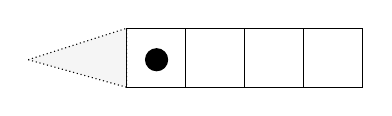
\begin{tikzpicture}
			\FIFODrawingFour
		\end{tikzpicture}
	};
%\draw[->, >=triangle 60,dashed] ($(channelThree)+(0,-1.5)$) -- (fifoTwo);
%\draw[->, >=triangle 60,dashed] ($(channelFour)+(0.1,0.6)$) -- ($(fifoTwo)+(0,0.2)$);
%\end{scope}
\node  (memDDR) at (10.5,0.5) {
		\begin{tikzpicture}
			\memoryDDRPointer
		\end{tikzpicture}
	};

    \node (legendStatic) at (5,-3.5){
                \resizebox{200pt}{!}{
                \begin{tikzpicture}
                        \legendApp
                \end{tikzpicture}}
        };

\draw [decorate,decoration={brace,amplitude=10pt,mirror,raise=4pt},yshift=0pt] (10.2,4) -- (10.2,0) node  [black,midway,xshift=0cm,yshift=-1cm] {};
\node (legChannel1) at (9.5,2) {};
\node(MRBleg) at ($(fifoTwo.north)+(0.3,0.2)$) {\Large $\channel_{\{1,2,3\}}$'s buffer};
\draw[->, >=triangle 60,dashed] ($(MRBleg.north)+(0.8,0)$) -- (legChannel1);
\node (leg) at (10.5,-3.5) {\Large \begin{tabular}{c}global memory \\ ($\GlobalMemory$) \end{tabular}};



}







